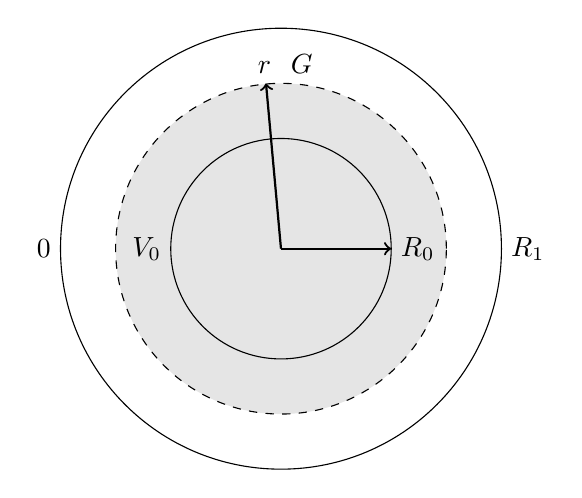
\begin{tikzpicture}[scale=0.7]
  \draw[dashed, fill=black!10]
    (0,0) circle [radius=3cm]
    ++ (0,3cm) node [above right] {$G$}
    node (G) [above left] {$r$}
  ;
  \draw[->, thick] (0,0) -- (G);
  \draw
    (0,0) circle [radius=2cm]
    ++ (2cm,0) node (R0) [right] {$R_0$}
    (0,0) ++ (-2cm,0) node  [left] {$V_0$}
  ;
  \draw[->, thick] (0,0) -- (R0);
  \draw
    (0,0) circle [radius=4cm]
    ++ (4cm,0) node (R1) [right] {$R_1$}
    (0,0) ++ (-4cm,0) node  [left] {$0$}
  ;
\end{tikzpicture}

